% Options for packages loaded elsewhere
\PassOptionsToPackage{unicode}{hyperref}
\PassOptionsToPackage{hyphens}{url}
%
\documentclass[
]{article}
\usepackage{lmodern}
\usepackage{amssymb,amsmath}
\usepackage{ifxetex,ifluatex}
\ifnum 0\ifxetex 1\fi\ifluatex 1\fi=0 % if pdftex
  \usepackage[T1]{fontenc}
  \usepackage[utf8]{inputenc}
  \usepackage{textcomp} % provide euro and other symbols
\else % if luatex or xetex
  \usepackage{unicode-math}
  \defaultfontfeatures{Scale=MatchLowercase}
  \defaultfontfeatures[\rmfamily]{Ligatures=TeX,Scale=1}
\fi
% Use upquote if available, for straight quotes in verbatim environments
\IfFileExists{upquote.sty}{\usepackage{upquote}}{}
\IfFileExists{microtype.sty}{% use microtype if available
  \usepackage[]{microtype}
  \UseMicrotypeSet[protrusion]{basicmath} % disable protrusion for tt fonts
}{}
\makeatletter
\@ifundefined{KOMAClassName}{% if non-KOMA class
  \IfFileExists{parskip.sty}{%
    \usepackage{parskip}
  }{% else
    \setlength{\parindent}{0pt}
    \setlength{\parskip}{6pt plus 2pt minus 1pt}}
}{% if KOMA class
  \KOMAoptions{parskip=half}}
\makeatother
\usepackage{xcolor}
\IfFileExists{xurl.sty}{\usepackage{xurl}}{} % add URL line breaks if available
\IfFileExists{bookmark.sty}{\usepackage{bookmark}}{\usepackage{hyperref}}
\hypersetup{
  pdftitle={First Implementation of QuickPay (2009-2012)},
  hidelinks,
  pdfcreator={LaTeX via pandoc}}
\urlstyle{same} % disable monospaced font for URLs
\usepackage[margin=1in]{geometry}
\usepackage{graphicx}
\makeatletter
\def\maxwidth{\ifdim\Gin@nat@width>\linewidth\linewidth\else\Gin@nat@width\fi}
\def\maxheight{\ifdim\Gin@nat@height>\textheight\textheight\else\Gin@nat@height\fi}
\makeatother
% Scale images if necessary, so that they will not overflow the page
% margins by default, and it is still possible to overwrite the defaults
% using explicit options in \includegraphics[width, height, ...]{}
\setkeys{Gin}{width=\maxwidth,height=\maxheight,keepaspectratio}
% Set default figure placement to htbp
\makeatletter
\def\fps@figure{htbp}
\makeatother
\setlength{\emergencystretch}{3em} % prevent overfull lines
\providecommand{\tightlist}{%
  \setlength{\itemsep}{0pt}\setlength{\parskip}{0pt}}
\setcounter{secnumdepth}{5}
\usepackage{booktabs,longtable,dcolumn} \usepackage{multirow,array} \usepackage{wrapfig,float} \floatplacement{figure}{H}

\title{First Implementation of QuickPay (2009-2012)}
\author{}
\date{\vspace{-2.5em}Mar 14, 2021}

\begin{document}
\maketitle

\hypertarget{delays-over-time}{%
\section{Delays over Time}\label{delays-over-time}}

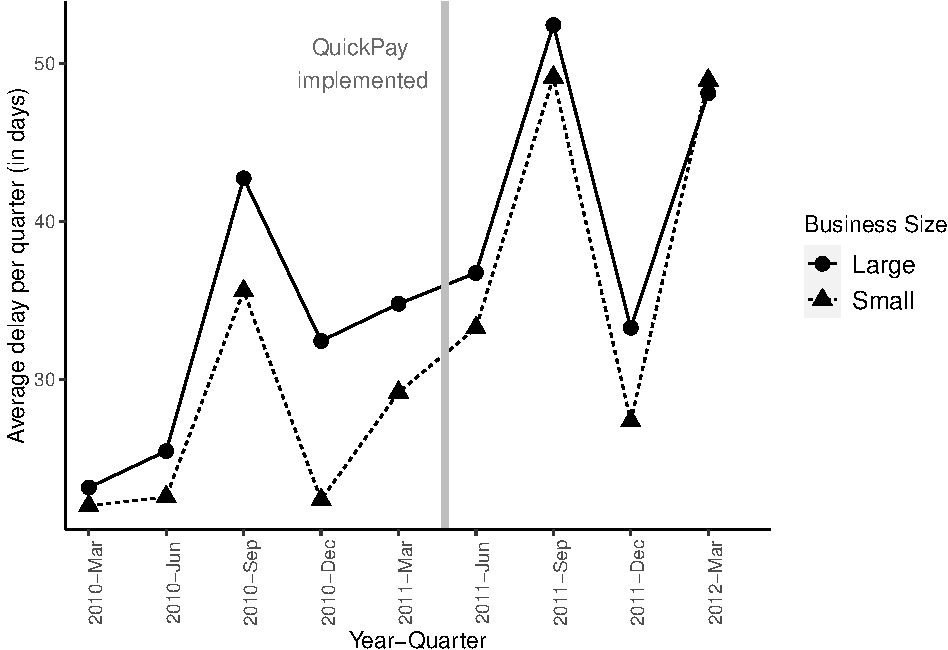
\includegraphics{qp_first_implementation_files/figure-latex/plot-1.pdf}

\hypertarget{notation}{%
\section{Notation}\label{notation}}

\begin{itemize}
\tightlist
\item
  Project \(i\), Year-Quarter \(t\)
\item
  \(X_i\) denotes project level controls: initial duration, initial
  budget, number of offers received
\item
  \(\mu_t,\theta_{firm},\lambda_{task}\): Year-Quarter, Firm, and
  Product/Service code Fixed effects
\item
  All continuous variables are winsorized at the 5\% level
  \[ Treat_i = \begin{cases} 1, \text{ if project } i \text{ is a small business}\\
  0, \text{ otherwise} \end{cases}\]
  \[ Post_t = \begin{cases} 1, \text{ if year-quarter } t > \text{ April 27, 2011}\\
  0, \text{ otherwise} \end{cases}\]
\end{itemize}

\hypertarget{parallel-trends-test}{%
\section{Parallel Trends Test}\label{parallel-trends-test}}

Let \(Time\) denote \(q\)-th quarter since the beginning of time
horizon. For \(Post_t =0\), we run the following regression:
\[ Delay_{it} = \alpha+\beta_0 Treat_i + \beta_1 (Treat_i \times Time) + \beta_2 X_i + \mu_t + \theta_{firm} + \lambda_{task} +\epsilon_{it}\]
The coefficient of interest is \(\beta_1\). If this is significant, we
would find evidence of a linear time trend before quickpay
implementation -- violating the parallel trends assumption.

\begin{table}[H] \centering 
  \caption{Linear Time Trend Before QuickPay} 
  \label{} 
\small 
\begin{tabular}{@{\extracolsep{5pt}}lc} 
\\[-1.8ex]\hline 
\hline \\[-1.8ex] 
 & \multicolumn{1}{c}{\textit{Dependent variable:}} \\ 
\cline{2-2} 
\\[-1.8ex] & $Delay_{it}$ (in days) \\ 
\hline \\[-1.8ex] 
 $Treat_i$ & $-$1.10 \\ 
  & (2.98) \\ 
  & \\ 
 $Treat_i \times Time$ & $-$0.01 \\ 
  & (0.49) \\ 
  & \\ 
\hline \\[-1.8ex] 
Fixed effects & Firm, Task, and Year-Quarter \\ 
Controls & Budget, Duration, Bids \\ 
Observations & 74,677 \\ 
R$^{2}$ & 0.14 \\ 
Adjusted R$^{2}$ & 0.03 \\ 
\hline 
\hline \\[-1.8ex] 
\textit{Note:}  & \multicolumn{1}{r}{$^{*}$p$<$0.1; $^{**}$p$<$0.05; $^{***}$p$<$0.01} \\ 
 & \multicolumn{1}{r}{Each observation is a project-quarter.} \\ 
 & \multicolumn{1}{r}{SEs are robust and clustered at the project level.} \\ 
 & \multicolumn{1}{r}{Observations are for quarters before quickpay.} \\ 
\end{tabular} 
\end{table}

\hypertarget{baseline-regressions}{%
\section{Baseline Regressions}\label{baseline-regressions}}

\[ Delay_{it} = \alpha+\beta_0 Treat_i + \beta_1 Post_t + \beta_2 (Treat_i \times Post_t) + \epsilon_{it}\]

\[ \begin{aligned} Delay_{it} &=& \alpha+\beta_0 Treat_i + \beta_1 Post_t + \beta_2 (Treat_i \times Post_t)\\
&+&  X_i + (Post_t \times X_i) + \mu_t + \theta_{firm} + \lambda_{task}+ \epsilon_{it}
\end{aligned}\]

\begin{table}[H] \centering 
  \caption{Quickpay 2009-2011} 
  \label{} 
\small 
\begin{tabular}{@{\extracolsep{-2pt}}lccc} 
\\[-1.8ex]\hline 
\hline \\[-1.8ex] 
\\[-1.8ex] & \multicolumn{3}{c}{$Delay_{it}$ (in days)} \\ 
\\[-1.8ex] & (1) & (2) & (3)\\ 
\hline \\[-1.8ex] 
 $Treat_i$ & $-$6.19$^{***}$ & $-$3.58$^{**}$ & $-$3.09$^{*}$ \\ 
  & (0.50) & (1.55) & (1.59) \\ 
  & & & \\ 
 $Post_t$ & 13.04$^{***}$ &  &  \\ 
  & (0.52) &  &  \\ 
  & & & \\ 
 $Treat_i \times Post_t$ & 3.35$^{***}$ & 6.88$^{***}$ & 6.83$^{***}$ \\ 
  & (0.73) & (0.91) & (0.92) \\ 
  & & & \\ 
 Constant & 33.00$^{***}$ &  &  \\ 
  & (0.36) &  &  \\ 
  & & & \\ 
\hline \\[-1.8ex] 
Year-Quarter Fixed Effects & No & Yes & Yes \\ 
Firm Fixed Effects & No & Yes & Yes \\ 
Task Fixed Effects & No & No & Yes \\ 
Duration, Budget, Bids & No & Yes & Yes \\ 
$Post_t \times$  (Duration, Budget, Bids) & No & Yes & Yes \\ 
Observations & 173,900 & 155,638 & 155,638 \\ 
R$^{2}$ & 0.01 & 0.11 & 0.12 \\ 
Adjusted R$^{2}$ & 0.01 & 0.05 & 0.05 \\ 
\hline 
\hline \\[-1.8ex] 
\textit{Note:}  & \multicolumn{3}{r}{$^{*}$p$<$0.1; $^{**}$p$<$0.05; $^{***}$p$<$0.01} \\ 
 & \multicolumn{3}{r}{Each observation is a project-quarter.} \\ 
 & \multicolumn{3}{r}{SEs are robust and clustered at the project level.} \\ 
\end{tabular} 
\end{table}

\hypertarget{contract-financing}{%
\section{Contract Financing}\label{contract-financing}}

\[ CF_i = \begin{cases} 1, \text{ if project } i \text{ receives contract financing}\\
0, \text{ otherwise} \end{cases}\]

\[ \begin{aligned}
Delay_{it} &=& \alpha+\beta_0 Treat_i + \beta_1 Post_t + \beta_2 (Treat_i \times Post_t) \\
&+&\beta_3 CF_i + \beta_4 (CF_i \times Post_t) + \beta_5 (Treat_i \times Post_t \times CF_i) \\ 
&+&X_i + (Post_t \times X_i) + \mu_t + \theta_{firm} + \lambda_{task}+ \epsilon_{it}
\end{aligned}\]

\begin{table}[H] \centering 
  \caption{Effect of Contract Financing: Quickpay 2009-2011} 
  \label{} 
\small 
\begin{tabular}{@{\extracolsep{-2pt}}lccc} 
\\[-1.8ex]\hline 
\hline \\[-1.8ex] 
\\[-1.8ex] & \multicolumn{3}{c}{$Delay_{it}$ (in days)} \\ 
\\[-1.8ex] & (1) & (2) & (3)\\ 
\hline \\[-1.8ex] 
 $Treat_i$ & $-$6.12$^{***}$ & $-$3.37$^{**}$ & $-$2.89$^{*}$ \\ 
  & (0.50) & (1.55) & (1.59) \\ 
  & & & \\ 
 $Post_t$ & 13.00$^{***}$ &  &  \\ 
  & (0.57) &  &  \\ 
  & & & \\ 
 $Treat_i \times Post_t$ & 1.53$^{**}$ & 5.89$^{***}$ & 5.90$^{***}$ \\ 
  & (0.78) & (1.00) & (1.01) \\ 
  & & & \\ 
 $CF_i$ & $-$3.97$^{***}$ & $-$4.68$^{***}$ & $-$4.76$^{***}$ \\ 
  & (0.61) & (0.81) & (0.82) \\ 
  & & & \\ 
 $Post_t \times CF_i$ & 0.72 & $-$0.20 & $-$0.37 \\ 
  & (1.13) & (1.31) & (1.32) \\ 
  & & & \\ 
 $Post_t \times CF_i \times Treat_i$ & 9.24$^{***}$ & 3.94$^{**}$ & 3.70$^{**}$ \\ 
  & (1.38) & (1.65) & (1.67) \\ 
  & & & \\ 
 Constant & 33.64$^{***}$ &  &  \\ 
  & (0.38) &  &  \\ 
  & & & \\ 
\hline \\[-1.8ex] 
Year-Quarter Fixed Effects & No & Yes & Yes \\ 
Firm Fixed Effects & No & Yes & Yes \\ 
Task Fixed Effects & No & No & Yes \\ 
Duration, Budget, Bids & No & Yes & Yes \\ 
$Post_t \times $  (Duration, Budget, Bids) & No & Yes & Yes \\ 
Observations & 173,900 & 155,638 & 155,638 \\ 
R$^{2}$ & 0.01 & 0.11 & 0.12 \\ 
Adjusted R$^{2}$ & 0.01 & 0.05 & 0.05 \\ 
\hline 
\hline \\[-1.8ex] 
\textit{Note:}  & \multicolumn{3}{r}{$^{*}$p$<$0.1; $^{**}$p$<$0.05; $^{***}$p$<$0.01} \\ 
 & \multicolumn{3}{r}{Each observation is a project-quarter.} \\ 
 & \multicolumn{3}{r}{SEs are robust and clustered at the project level.} \\ 
\end{tabular} 
\end{table}

\hypertarget{receives-financial-aid}{%
\section{Receives Financial Aid}\label{receives-financial-aid}}

\[ FinancialAid = \begin{cases} 1, \text{ if firm receives grants or is a c8A participant}\\
0, \text{ otherwise} \end{cases}\]

\[ \begin{aligned}
Delay_{it} &=& \alpha+\beta_0 Treat_i + \beta_1 Post_t + \beta_2 (Treat_i \times Post_t) +\beta_3 FinancialAid \\
&+& \beta_4 (FinancialAid \times Post_t) + \beta_5 (Treat_i \times Post_t \times FinancialAid) \\ 
&+&X_i + (Post_t \times X_i) + \mu_t + \theta_{firm} + \lambda_{task}+ \epsilon_{it}
\end{aligned}\]

\begin{table}[H] \centering 
  \caption{Effect of Grants or C8A Participant: Quickpay 2009-2011} 
  \label{} 
\small 
\begin{tabular}{@{\extracolsep{-2pt}}lccc} 
\\[-1.8ex]\hline 
\hline \\[-1.8ex] 
\\[-1.8ex] & \multicolumn{3}{c}{$Delay_{it}$ (in days)} \\ 
\\[-1.8ex] & (1) & (2) & (3)\\ 
\hline \\[-1.8ex] 
 $Treat_i$ & $-$6.96$^{***}$ & $-$3.15$^{**}$ & $-$2.63$^{*}$ \\ 
  & (0.51) & (1.55) & (1.59) \\ 
  & & & \\ 
 $Post_t$ & 12.89$^{***}$ &  &  \\ 
  & (0.53) &  &  \\ 
  & & & \\ 
 $Treat_i \times Post_t$ & 3.43$^{***}$ & 5.65$^{***}$ & 5.57$^{***}$ \\ 
  & (0.77) & (0.98) & (0.99) \\ 
  & & & \\ 
 $FinancialAid$ & 5.72$^{***}$ & 1.36 & 0.45 \\ 
  & (0.70) & (1.39) & (1.42) \\ 
  & & & \\ 
 $Post_t \times FinancialAid$ & 1.94 & 4.06$^{*}$ & 3.93$^{*}$ \\ 
  & (1.61) & (2.10) & (2.12) \\ 
  & & & \\ 
 $Post_t \times FinancialAid \times Treat_i$ & $-$1.80 & 2.51 & 2.75 \\ 
  & (1.73) & (2.46) & (2.50) \\ 
  & & & \\ 
 Constant & 32.42$^{***}$ &  &  \\ 
  & (0.37) &  &  \\ 
  & & & \\ 
\hline \\[-1.8ex] 
Year-Quarter Fixed Effects & No & Yes & Yes \\ 
Firm Fixed Effects & No & Yes & Yes \\ 
Task Fixed Effects & No & No & Yes \\ 
Duration, Budget, Bids & No & Yes & Yes \\ 
$Post_t \times$  (Duration, Budget, Bids) & No & Yes & Yes \\ 
Observations & 173,900 & 155,638 & 155,638 \\ 
R$^{2}$ & 0.01 & 0.11 & 0.12 \\ 
Adjusted R$^{2}$ & 0.01 & 0.05 & 0.05 \\ 
\hline 
\hline \\[-1.8ex] 
\textit{Note:}  & \multicolumn{3}{r}{$^{*}$p$<$0.1; $^{**}$p$<$0.05; $^{***}$p$<$0.01} \\ 
 & \multicolumn{3}{r}{Each observation is a project-quarter.} \\ 
 & \multicolumn{3}{r}{SEs are robust and clustered at the project level.} \\ 
\end{tabular} 
\end{table}

\hypertarget{receives-contracts-and-financial-aid}{%
\section{Receives Contracts and Financial
Aid}\label{receives-contracts-and-financial-aid}}

\[ CFA = \begin{cases} 1, \text{ if firm receives "contracts and grants"}\\ 
                       \text{or grants or is a c8A participant}\\
0, \text{ otherwise} \end{cases}\]

\[ \begin{aligned}
Delay_{it} &=& \alpha+\beta_0 Treat_i + \beta_1 Post_t + \beta_2 (Treat_i \times Post_t) +\beta_3 CFA \\
&+& \beta_4 (CFA \times Post_t) + \beta_5 (Treat_i \times Post_t \times CFA) \\ 
&+&X_i + (Post_t \times X_i) + \mu_t + \theta_{firm} + \lambda_{task}+ \epsilon_{it}
\end{aligned}\]

\begin{table}[H] \centering 
  \caption{Effect of Contracts, Grants, or C8A Participant: Quickpay 2009-2011} 
  \label{} 
\small 
\begin{tabular}{@{\extracolsep{-2pt}}lccc} 
\\[-1.8ex]\hline 
\hline \\[-1.8ex] 
\\[-1.8ex] & \multicolumn{3}{c}{$Delay_{it}$ (in days)} \\ 
\\[-1.8ex] & (1) & (2) & (3)\\ 
\hline \\[-1.8ex] 
 $Treat_i$ & $-$6.68$^{***}$ & $-$3.19$^{**}$ & $-$2.71$^{*}$ \\ 
  & (0.51) & (1.55) & (1.59) \\ 
  & & & \\ 
 $Post_t$ & 12.17$^{***}$ &  &  \\ 
  & (0.55) &  &  \\ 
  & & & \\ 
 $Treat_i \times Post_t$ & 4.19$^{***}$ & 5.71$^{***}$ & 5.84$^{***}$ \\ 
  & (0.79) & (1.02) & (1.03) \\ 
  & & & \\ 
 $CFA$ & 4.90$^{***}$ & $-$5.44$^{***}$ & $-$5.92$^{***}$ \\ 
  & (0.62) & (1.78) & (1.80) \\ 
  & & & \\ 
 $Post_t \times CFA$ & 3.91$^{***}$ & 5.00$^{***}$ & 5.83$^{***}$ \\ 
  & (1.21) & (1.60) & (1.64) \\ 
  & & & \\ 
 $Post_t \times CFA \times Treat_i$ & $-$4.04$^{***}$ & 2.60 & 1.61 \\ 
  & (1.38) & (2.12) & (2.16) \\ 
  & & & \\ 
 Constant & 32.18$^{***}$ &  &  \\ 
  & (0.37) &  &  \\ 
  & & & \\ 
\hline \\[-1.8ex] 
Year-Quarter Fixed Effects & No & Yes & Yes \\ 
Firm Fixed Effects & No & Yes & Yes \\ 
Task Fixed Effects & No & No & Yes \\ 
Duration, Budget, Bids & No & Yes & Yes \\ 
$Post_t \times$  (Duration, Budget, Bids) & No & Yes & Yes \\ 
Observations & 173,900 & 155,638 & 155,638 \\ 
R$^{2}$ & 0.01 & 0.11 & 0.12 \\ 
Adjusted R$^{2}$ & 0.01 & 0.05 & 0.05 \\ 
\hline 
\hline \\[-1.8ex] 
\textit{Note:}  & \multicolumn{3}{r}{$^{*}$p$<$0.1; $^{**}$p$<$0.05; $^{***}$p$<$0.01} \\ 
 & \multicolumn{3}{r}{Each observation is a project-quarter.} \\ 
 & \multicolumn{3}{r}{SEs are robust and clustered at the project level.} \\ 
\end{tabular} 
\end{table}

\hypertarget{firms-rank-order}{%
\section{Firm's rank order}\label{firms-rank-order}}

\begin{itemize}
\tightlist
\item
  Consider a project \(i\) of firm \(f\) in quarter \(t\).
\item
  Let \(\Pi_{f,2010}\) denote all projects of firm \(f\) in Fiscal Year
  2010.
\item
  Consider
  \(\rho_f = \sum_{i \in \Pi_{f,2010}} (Treat_i \times FAO_{if})/Sales_{f,\text{2010}}\)
  as the fraction of revenue a firm earns from small government
  projects.
\item
  Let \(\Theta_f = rank(\rho_f)/N\) where \(rank(\rho_f)\) is the rank
  statistic of \(\rho_{f}\) and \(N = \text{number of firms}.\) For
  example, \(rank(\rho_f)=1\) if
  \(\rho_f=\min(\rho_1,\rho_2,\ldots,\rho_N)\).
\item
  Put simply, \(\Theta_f\) is a firm's rank order based on the fraction
  of revenue it earned from small government projects in FY 2010.
\end{itemize}

\hypertarget{portfolio-effects-discrete}{%
\subsection{Portfolio Effects:
Discrete}\label{portfolio-effects-discrete}}

\begin{itemize}
\tightlist
\item
  See
  \href{https://github.com/QuickPay-Operational-Performance/Data-and-code/blob/master/notes/Portfolio\%20model\%2B0308.pdf}{Jie's
  notes} for details.
\item
  Let \(Rank_f^{(k)}\) be an indicator for firm being in the k-th
  tercile of \(Rank\).Define:

  \begin{itemize}
  \tightlist
  \item
    \(Medium_i = Treat_i * Rank_f^{(2)}\)
  \item
    \(High_i = Treat_i * Rank_f^{(3)}\)
  \end{itemize}
\end{itemize}

\[\begin{aligned} Delay_{it}&=&\beta_0+\beta_1 Treat_i + \beta_2 Medium_i+\beta_3 High_i +\beta_4 Post_t\\ && +\beta_5( Treat_i\times Post_t) + \beta_6(Medium_i\times Post_t) + \beta_7(High_i\times Post_t) + \epsilon_{it} \end{aligned}\]

\begin{table}[H] \centering 
  \caption{Discrete Portfolio Effects: Quickpay 2009-2011} 
  \label{} 
\small 
\begin{tabular}{@{\extracolsep{-2pt}}lccccc} 
\\[-1.8ex]\hline 
\hline \\[-1.8ex] 
\\[-1.8ex] & \multicolumn{5}{c}{$Delay_{it}$ (in days)} \\ 
\\[-1.8ex] & (1) & (2) & (3) & (4) & (5)\\ 
\hline \\[-1.8ex] 
 $Treat_i$ & 2.85$^{**}$ & $-$0.51 & $-$0.37 & 0.38 & $-$6.90 \\ 
  & (1.37) & (1.54) & (1.55) & (1.64) & (4.47) \\ 
  & & & & & \\ 
 $Medium_i$ & $-$2.92$^{**}$ & $-$1.11 & $-$1.32 & $-$0.60 & 12.24$^{**}$ \\ 
  & (1.40) & (1.56) & (1.57) & (1.63) & (6.17) \\ 
  & & & & & \\ 
 $High_i$ & $-$3.26$^{**}$ & 0.09 & $-$0.07 & 1.04 & $-$3.11 \\ 
  & (1.31) & (1.49) & (1.50) & (1.58) & (6.04) \\ 
  & & & & & \\ 
 $Post_t$ & 15.67$^{***}$ & 6.87$^{***}$ &  &  &  \\ 
  & (1.05) & (1.83) &  &  &  \\ 
  & & & & & \\ 
 $Treat_i \times Post_t$ & $-$2.42 & 2.15 & 1.26 & 1.32 & 7.32$^{**}$ \\ 
  & (2.04) & (2.36) & (2.39) & (2.43) & (3.16) \\ 
  & & & & & \\ 
 $Treat_i \times Post_t \times Medium_i$ & 4.28$^{**}$ & 1.54 & 2.31 & 2.45 & 0.10 \\ 
  & (2.09) & (2.38) & (2.41) & (2.45) & (3.22) \\ 
  & & & & & \\ 
 $Treat_i \times Post_t \times High_i$ & 6.76$^{***}$ & 3.46 & 4.16$^{*}$ & 3.58 & $-$1.27 \\ 
  & (1.97) & (2.28) & (2.31) & (2.35) & (3.07) \\ 
  & & & & & \\ 
 Constant & 27.08$^{***}$ & 46.30$^{***}$ &  &  &  \\ 
  & (0.71) & (1.16) &  &  &  \\ 
  & & & & & \\ 
\hline \\[-1.8ex] 
Duration, Budget, Bids & No & Yes & Yes & Yes & Yes \\ 
$Post_t \times$  (Duration, Budget, Bids) & No & Yes & Yes & Yes & Yes \\ 
Year-Quarter Fixed Effects & No & No & Yes & Yes & Yes \\ 
Task Fixed Effects & No & No & No & Yes & Yes \\ 
Firm Fixed Effects & No & No & No & No & Yes \\ 
Observations & 71,753 & 63,216 & 63,216 & 63,216 & 63,216 \\ 
R$^{2}$ & 0.01 & 0.02 & 0.03 & 0.06 & 0.12 \\ 
Adjusted R$^{2}$ & 0.01 & 0.02 & 0.03 & 0.04 & 0.04 \\ 
\hline 
\hline \\[-1.8ex] 
\textit{Note:}  & \multicolumn{5}{r}{$^{*}$p$<$0.1; $^{**}$p$<$0.05; $^{***}$p$<$0.01} \\ 
 & \multicolumn{5}{r}{Each observation is a project-quarter.} \\ 
 & \multicolumn{5}{r}{SEs are robust and clustered at the project level.} \\ 
\end{tabular} 
\end{table}

\hypertarget{portfolio-effects-continuous}{%
\subsection{Portfolio Effects:
Continuous}\label{portfolio-effects-continuous}}

\begin{itemize}
\tightlist
\item
  See
  \href{https://github.com/QuickPay-Operational-Performance/Data-and-code/blob/master/notes/Portfolio\%20model\%2B0308.pdf}{Jie's
  notes} for details.
\item
  Define \(\theta_i = Treat_i*Rank_f\)
\end{itemize}

\[ \begin{aligned} Delay_{it}&=&\beta_0+\beta_1 Treat_i + \beta_2 \theta_i+\beta_3 \theta_i^2+\beta_4 Post_t\\&& + \beta_5 (Treat_i\times Post_t) + \beta_6 (\theta_i\times Post_t) +\beta_7 (\theta_i^2\times Post_t)+\epsilon_{it} \end{aligned} \]

\begin{table}[H] \centering 
  \caption{Discrete Portfolio Effects: Quickpay 2009-2011} 
  \label{} 
\small 
\begin{tabular}{@{\extracolsep{-2pt}}lccccc} 
\\[-1.8ex]\hline 
\hline \\[-1.8ex] 
\\[-1.8ex] & \multicolumn{5}{c}{$Delay_{it}$ (in days)} \\ 
\\[-1.8ex] & (1) & (2) & (3) & (4) & (5)\\ 
\hline \\[-1.8ex] 
 $Treat_i$ & $-$1.44 & $-$4.54 & $-$4.12 & $-$2.25 & $-$19.01$^{**}$ \\ 
  & (2.52) & (2.79) & (2.80) & (2.88) & (8.36) \\ 
  & & & & & \\ 
 $\theta_i$ & 15.63$^{*}$ & 12.24 & 11.06 & 8.21 & 92.44$^{***}$ \\ 
  & (8.14) & (8.85) & (8.89) & (9.06) & (34.90) \\ 
  & & & & & \\ 
 $\theta_i^2$ & 15.67$^{***}$ & 6.85$^{***}$ &  &  &  \\ 
  & (1.05) & (1.83) &  &  &  \\ 
  & & & & & \\ 
 $Post_t$ & $-$3.83 & 2.64 & 1.05 & 0.34 & 9.39 \\ 
  & (3.74) & (4.31) & (4.38) & (4.45) & (5.79) \\ 
  & & & & & \\ 
 $Treat_i \times Post_t$ & 4.16 & $-$3.40 & $-$0.02 & 3.49 & $-$4.73 \\ 
  & (12.19) & (13.75) & (13.98) & (14.13) & (17.63) \\ 
  & & & & & \\ 
 $\theta_i \times Post_t$ & $-$16.17$^{**}$ & $-$8.85 & $-$8.10 & $-$5.07 & $-$88.48$^{***}$ \\ 
  & (6.56) & (7.11) & (7.15) & (7.30) & (31.25) \\ 
  & & & & & \\ 
 $\theta_i^2 \times Post_t$ & 4.91 & 6.92 & 4.92 & 1.51 & 1.46 \\ 
  & (9.87) & (11.09) & (11.27) & (11.38) & (13.78) \\ 
  & & & & & \\ 
 Constant & 27.08$^{***}$ & 46.30$^{***}$ &  &  &  \\ 
  & (0.71) & (1.16) &  &  &  \\ 
  & & & & & \\ 
\hline \\[-1.8ex] 
Duration, Budget, Bids & No & Yes & Yes & Yes & Yes \\ 
$Post_t \times$  (Duration, Budget, Bids) & No & Yes & Yes & Yes & Yes \\ 
Year-Quarter Fixed Effects & No & No & Yes & Yes & Yes \\ 
Task Fixed Effects & No & No & No & Yes & Yes \\ 
Firm Fixed Effects & No & No & No & No & Yes \\ 
Observations & 71,753 & 63,216 & 63,216 & 63,216 & 63,216 \\ 
R$^{2}$ & 0.01 & 0.02 & 0.03 & 0.06 & 0.12 \\ 
Adjusted R$^{2}$ & 0.01 & 0.02 & 0.03 & 0.04 & 0.04 \\ 
\hline 
\hline \\[-1.8ex] 
\textit{Note:}  & \multicolumn{5}{r}{$^{*}$p$<$0.1; $^{**}$p$<$0.05; $^{***}$p$<$0.01} \\ 
 & \multicolumn{5}{r}{Each observation is a project-quarter.} \\ 
 & \multicolumn{5}{r}{SEs are robust and clustered at the project level.} \\ 
\end{tabular} 
\end{table}

--\textgreater{}

--\textgreater{} --\textgreater{} --\textgreater{} --\textgreater{}
--\textgreater{}

\end{document}
